\documentclass[a4paper]{article}

%% Language and font encodings
\usepackage[spanish,es-tabla]{babel}
\usepackage[utf8x]{inputenc}
\usepackage{natbib}
\usepackage{booktabs}
\usepackage{tabu}
\usepackage[T1]{fontenc}
\usepackage{subcaption}
\usepackage{float}
\usepackage{amssymb}
\usepackage{multirow}
\usepackage{comment}

%% Sets page size and margins
\usepackage[a4paper,top=3cm,bottom=2cm,left=3cm,right=3cm,marginparwidth=1.75cm]{geometry}

%% Useful packages
\usepackage{amsmath}
\usepackage{graphicx}
%\usepackage{apacite}
\usepackage[colorinlistoftodos]{todonotes}
\usepackage[colorlinks=true, allcolors=blue]{hyperref}

\renewcommand{\labelenumii}{\theenumii}
\renewcommand{\theenumii}{\theenumi.\arabic{enumii}.}

\title{Desarrollo de una Aplicación Web para la Detección de Neoantígenos en el Marco de Desarrollo de Vacunas Personalizadas para Tratar el Cáncer }
\author{Vicente Machaca Arceda y Richart  Escobedo Quispe}
\date{\today}

\begin{document}
	

	
	
	
	
	
	
	
	\maketitle

\section{Título}

Desarrollo de una Aplicación Web para la Detección de Neoantígenos en el Marco de Desarrollo de Vacunas Personalizadas para Tratar el Cáncer

\section{Lineas de investigación}
Inteligencia Artificial y Tecnologías de la Programación.

 
	\section{Breve estado de la cuestión}
	
	El cáncer representa el mayor problema de salud mundial y es la principal causa de muerte, con alrededor de un millón de fallecimientos reportados en 2020. Además, los métodos tradicionales basados en cirugías, radioterapias y quimioterapias tienen baja efectividad \citep{peng2019neoantigen}. En este contexto, surge el desarrollo de la inmunoterapia de cáncer, que tiene como objetivo estimular el sistema inmunológico de un paciente \citep{borden2022cancer}. En esta área, ha emergido la investigación basada en la detección de neoantígenos, hay tres tratamientos: vacunas personalizadas, terapias de células T adoptivas e inhibidores de puntos de control inmunológico. De los métodos mencionados anteriormente, se considera que el desarrollo de vacunas personalizadas  tiene la mayor probabilidad de éxito \citep{borden2022cancer}.\\

Los neoantígenos son péptidos mutados específicos del tumor y se consideran las principales causas de una respuesta inmune \citep{borden2022cancer,chen2021challenges,gopanenko2020main}. El objetivo es entrenar los linfocitos (células T) de un paciente para que reconozcan los neoantígenos y activen el sistema inmunológico \citep{de2020neoantigen,peng2019neoantigen}. El ciclo de vida de un neoantígeno para las células con núcleo se puede resumir de la siguiente manera. Primero, una proteína se degrada en péptidos (posibles neoantígenos) en el citoplasma. A continuación, los péptidos se unen al Complejo Mayor de Histocompatibilidad (MHC), conocido como unión péptido-MHC (pMHC \textit{binding}). Luego, este compuesto sigue una vía hasta llegar a la membrana celular (pMHC \textit{presentation}). Finalmente, el pMHC es reconocido por el \textit{T-cell Receptor} (TCR), lo que desencadena el sistema inmunológico. En este contexto, este proyecto se centra en la predicción de la union del MHC con un péptido (pMHC). Si la unión ocurre, entonces el péptido en cuestión podría ser considerado un neoantígeno. \\



Referente a la 	predicción de la unión pMHC, existen dos enfoques: \textit{allele-specific} y \textit{pan-specific}; el primero desarrolla modelos por cada tipo de MHC, si consideramos que existen miles de variantes de MHC, este enfoque no es viable; el segundo enfoque \textit{allele-specific}, desarrolla un solo modelo para predecir la unión pMHC. En los siguientes párrafos, explicaremos brevemente los principales trabajos desarrollados hasta la actualidad.\\
	
	NetMHCPan4.1 \citep{reynisson2020netmhcpan} es un método 	\textit{pan-specific} considerado como una línea base para la predicción de pMHC-I. Este método utiliza Redes Neuronales Artificiales (ANN). Mejoró sus versiones anteriores al aumentar el conjunto de datos de entrenamiento con 13245212 puntos de datos que cubren 250 moléculas distintas de MHC-I; además, el modelo se actualizó de NN\_align a NN\_alignMA \citep{alvarez2019nnalign_ma}. Además, MHCflurry2.0 \citep{o2020mhcflurry} es otro método de vanguardia; utiliza un predictor de afinidad de unión pan-allelic, un predictor de presentación de antígeno independiente del allele y utiliza datos de Espectrometría de Masas (MS); después de experimentos, MHCflurry2.0 superó a NetMHCpan4.0. En cuanto a la predicción \textit{pan-specific} de pMHC-II, NetMHCIIpan4.0 \citep{reynisson2020netmhcpan} utilizó desconvolución de motif y datos de \textit{eluted ligands} por MS con 4086230 puntos de datos que cubren un total de 116 MHC-II distintos. Por otro lado, NetMHC4.0 \citep{andreatta2016gapped} es \textit{allele-specific}; actualizó sus versiones anteriores, agregando \textit{padding} a los aminoácidos y utilizó ANNs. \\

Los \textit{transformers} se consideran una revolución en la inteligencia artificial y se han aplicado con éxito en varias tareas de procesamiento del lenguaje natural (NLP, por sus siglas en inglés) \citep{patwardhan2023transformers}. Además, estos modelos se han utilizado en la detección de neoantígenos, centrándose en la predicción del enlace pMHC. Por ejemplo, BERTMHC \citep{cheng2021bertmhc} es un método 	\textit{pan-specific} para predecir el enlace pMHC-II; utiliza una arquitectura BERT y transfer learning de \textit{Tasks Assessing Protein Embedding}s (TAPE) \citep{rao2019evaluating}. Los autores aplican una \textit{mean pooling} seguida de una capa \textit{Fully Connected} (FC) después del modelo TAPE. En los experimentos, BERTMHC superó a NetMHCIIpan3.2 y PUFFIN. Además, ImmunoBERT \citep{gasser2021interpreting} también utilizó transfer learning de TAPE; sin embargo, los autores se enfocaron en la predicción de pMHC-I.\\

Además, MHCRoBERTa \citep{wang2022mhcroberta} y HLAB \citep{zhang2022hlab} también utilizaron \textit{transfer learning}. MHCRoBERTa utilizó entrenamiento auto-supervisado a partir de las bases de datos UniProtKB y Swiss-prot; luego, aplicaron \textit{fine-tunning} con datos de IEDB \citep{vita2019immune}. MHCRoBERTa superó a NetMHCpan4.0 y MHCflurry2.0 en SRCC. Por otro lado, HLAB \citep{zhang2022hlab} utilizó \textit{transfer learning} de ProtBert-BFD \citep{elnaggar2021prottrans}; utilizó un modelo BiLSTM en cascada. Además, en el \textit{allele} HLA-A*01:01, HLAB superó ligeramente a los métodos de vanguardia, incluido NetMHCpan4.1, en al menos 0.0230 en AUC y 0.0560 en precisión. Luego, nosotros hemos validado el uso de BERT y \textit{transfer learning} \citep{arceda2023neoantigen}.\\

Luego, TransPHLA \citep{chu2022transformer} es un método \textit{allele-specific} que aplica \textit{self-attention} a los péptidos. Los autores desarrollaron AOMP, que toma la unión de pMHC como entrada y devuelve péptidos mutantes con mayor afinidad hacia el \textit{allele} MHC. Además, TransPHLA superó a los métodos de vanguardia, incluido NetMHCpan4.1, y es efectivo para cualquier longitud de péptido y MHC, y es más rápido para hacer predicciones. Además, el método DapNet-HLA \textit{allele-specific} \citep{jing2023dapnet} obtuvo resultados interesantes, utilizó un conjunto de datos adicional (Swiss-Prot) para muestras negativas y combinó las ventajas de CNN, SENet (para agrupamiento) y LSTM. La propuesta obtuvo puntuaciones altas; sin embargo, el método no se comparó con métodos de vanguardia. Finalmente, nosotros en un trabajo anterior hemos desarrollado un \textit{review} donde se detalla las principales ventajas y limitaciones de este problema \citep{machaca2023deep}.\\


Finalmente, debido a la complejidad del proceso y la gran cantidad de métodos desarrollados, se ha desarrollado software y \textit{pipelines} que pretenden facilitar el uso de estas herramientas. Entre las más recientes tenemos: Somaticseq \citep{fang2015ensemble}, NeoPredPipe \citep{schenck2019neopredpipe}, CloudNeo \citep{bais2017cloudneo}, MuPeXI \citep{bjerregaard2017mupexi}, NeoepitopePred \citep{tran2015immunogenicity}, Neoepiscope \citep{yossef2018enhanced}, pVACtools \citep{hundal2020pvactools}  y NeoFuse \citep{gros2016prospective}. Estas herramientas en su mayoría toman como entrada archivos VCF y archivos de alineamiento Bam, para la detección de mutaciones (inserciones, eliminaciones y fusión de genes) y posibles neo antígenos. 




\section{Planteamiento del problema}

Menos del 5\% de neoantígenos detectados llegan a la membrana y activan el sistema immune \citep{de2020neoantigen, mill2022neoms, bulik2019deep, bassani2015mass, yadav2014predicting}. Además, existen herramientas con buen desempeño en el problema de pMHC \textit{binding}, pero con resultados pobres en  pMHC \textit{presentation} \citep{bulik2019deep}. En este contexto, esta investigación se enfoca en la predicción de la unión pMHC. Este problema se puede representar como un problema de clasificación binaria, tomando un péptido y el MHC como entrada. Estos son secuencias de aminoácidos, el péptido se pueden representar como: $p = \{ A, ... , Q \}$ y el MHC como: $q = \{ A, N, ... ,Q, E, G \}$. Luego, tenemos que  predecir si $p$ y $q$ pueden enlazarse. %Posteriormente, debemos predecir el enlace pMHC-TCR, el complejo pMHC se puede representar como la concatenación de $p$ y $q$, mientras que que para el caso del TCR, se considera solo la elice $\alpha$ de su proteína, que viene a ser representada como otra secuencia de aminoácidos $r = \{  N, ... ,Q, E \}$. Finalmente, debemos predecir si la concatenación de las secuencias $p$ y $q$ se enlaza con la secuencia $r$.



	
\section{Objetivos de la investigación}
	
	\subsection{Objetivo general}
	
	Desarrollar una aplicación Web para la detección de neoantígenos en el marco del desarrollo de vacunas personalizadas para tratar el Cáncer.
	
	\subsection{Objetivos específicos}
	\begin{enumerate}
		\item Implementar un método basado en \textit{transformers} y \textit{transfer learning} para predecir la unión pMHC.	
		\item Comparar los resultados del método propuesto con NetMHCpan4.1.
		\item Implementar la aplicación Web para la detección de neoantígenos.
	

		

		
	\end{enumerate}

	
\section{Importancia de la investigación}

El cáncer es el mayor problema de salud mundial; sin embargo, los métodos tradicionales basados en cirugías, radioterapias y quimioterapias tienen baja efectividad \citep{peng2019neoantigen}. En este contexto, los neoantígenos son factores clave en el desarrollo de vacunas contra el Cáncer  \citep{borden2022cancer,chen2021challenges,gopanenko2020main}. Si se logra desarrollar un método con un buen desempeño, la inmunoterapia del cáncer basada en el desarrollo de vacunas personalizadas, podría utilizarse como alternativa a otros métodos como radioterapias y quimioterapias. \\

En el área de la inteligencia artificial y específicamente en el tópico de \textit{deep learning}, el desarrollo de un método basado en \textit{transformers} y \textit{transfer learning}, representa una contribución importante  y demuestra que este tipo de modelos no solo pueden utilizarse en campos del procesamiento natural del lenguaje (como lo hace chatGPT) sino también en otros ámbitos como la Immunoinformática.\\

Finalmente, tener una aplicación Web desarrollada por la universidad La Salle, realza el nombre de la universidad y la iguala a otras universidades que también desarrollan aplicaciones basadas en inteligencia artificial para solucionar  problemas interdisciplinarios.


\section{Posibles soluciones y consecuencias de la investigación}

Entre las consecuencias de la investigación tenemos: (1) una publicación con el método propuesto para la predicción de la unión pMHC y (2) una aplicación Web para la predicción de la unión pMHC. Luego, esta investigación abre las puertas para futuros proyectos que involucren el desarrollo de un \textit{pipeline} para la detección de neoantígenos, pero esta vez tomando como entrada una secuencia de ADN. Otro futuro proyecto de mayor envergadura involucra un trabajo interdisciplinario con biotecnólogos, biólogos y oncólogos; con el objetivo de desarrollar vacunas personalizadas para tratar el Cáncer. 

\section{Diseño y secuencia lógica de la investigación} 

Hemos dividido la propuesta en dos partes: la primera se basa en el desarrollo de un modelo de \textit{deep learning} basado en \textit{transformers} y \textit{transfer learning} para la predicción de la unión pMHC. Actualmente, ya tenemos resultados preliminares con un desempeño comparable a NetMHCpan4.1 (\textit{state-of-art method}) \citep{arceda2023neoantigen} y adicionalmente, hemos desarrollado un \textit{review} sobre los principales métodos del estado del arte \citep{machaca2023deep}. En la segunda parte del proyecto, se propone desarrollar la aplicación Web para la detección de neoantígenos, enfocados en la predicción de la unión pMHC.

\subsection{Desarrollo del modelo de inteligencia artificial}

En este proyecto, se propone utilizar una arquitectura BERT con \textit{transfer learning}. Analizamos alternativas como TAPE \citep{rao2019evaluating}, ProtBERT-BFD \citep{elnaggar2021prottrans}, ESM-1b \citep{rives2021biological} y ESM2 \citep{lin2023evolutionary} cada una con 92 millones, 420 millones, 650 millones y 15 billones de parámetros respectivamente. TAPE fue entrenado con 30 millones de proteínas, ProtBERT-BFD con 2122 millones de proteínas y 250 millones de proteínas para ESM-1b. Además, ESM-1b obtuvo mejores resultados en precisión de contacto que TAPE y ProtBERT-BFD \citep{rives2021biological}; sin embargo, ya contamos la versión nueva ESM2 \citep{lin2023evolutionary}.\\

Además, HLAB \citep{zhang2022hlab} propuso el uso de ProtBERT-BFD \citep{elnaggar2021prottrans} con un modelo BiLSTM en cascada y superó a NetMHCpan4.1 (método de vanguardia) en el \textit{allele} HLA-A*01:01. Por lo tanto, en este proyecto, proponemos utilizar el modelo preentrenado ESM2 \citep{lin2023evolutionary} con un capa BiLSTM  similar a HLAB \citep{zhang2022hlab}. Para el \textit{fine-tuning}, utilizaremos conjuntos de datos de NetMHCpan4.1 y NetMHCIIpan4.0.\\

En resumen, en la Figura. \ref{fig:proposal}, presentamos la propuesta: primero, se concatenan y se aplica \textit{padding} al péptido y la pseudo secuencia MHC; en segundo lugar, utilizamos el modelo \textit{transformer} ESM2 para obtener una nueva representación de los aminoácidos; finalmente, utilizamos un BiLSTM para predecir el enlace pMHC. 





\begin{figure}[H]
	\centering
	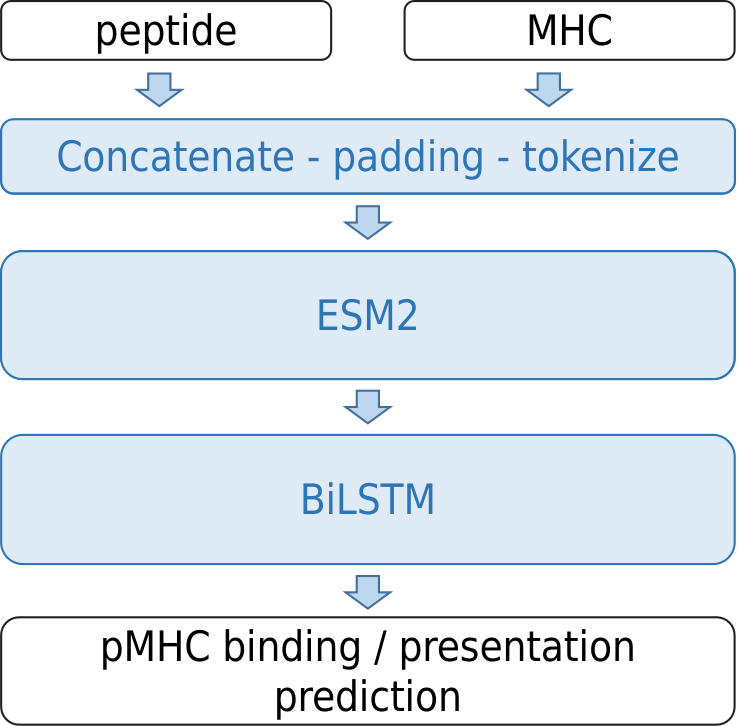
\includegraphics[width=0.35\textwidth]{img/neoantigen/proposal1}
	\caption{Propuesta: Utilizamos el modelo de transformer ESM2 seguido de BiLSTM para predecir el enlace pMHC.}
	\label{fig:proposal}
\end{figure}

\subsection{Desarrollo de la aplicación Web}

La aplicación Web se desarrollará para que un usuario pueda realizar predicciones de la unión pMHC. La página Web tomará como entrada un conjunto de péptidos y un tipo de MHC. Luego, retornará y mostrará que péptidos pueden unirse a dicho MHC y por lo tanto se les considera posibles neoantígenos.\\

Referente a las tecnologías a utilizar: para el \textit{BackEnd}, se utilizará el \textit{framework} Express.js de Javascript y el gestor de base de datos Mongo. Para el \textit{FrontEnd}, se propone utilizar Next.js. Se han seleccionado estas tecnologías debido a su versatilidad y la enorme documentación que presentan. La Figura \ref{fig:arquitectura} anterior, muestra el nodo del FrontEnd donde se tiene la interfaz de un navegador web responsivo, consumiendo el servicio disponible desde el BackEnd. En la implementación la aplicación web en NodeJS Express y la base de datos Mongo se encuentran en el mismo servidor.


\begin{figure}[H]
	\centering
	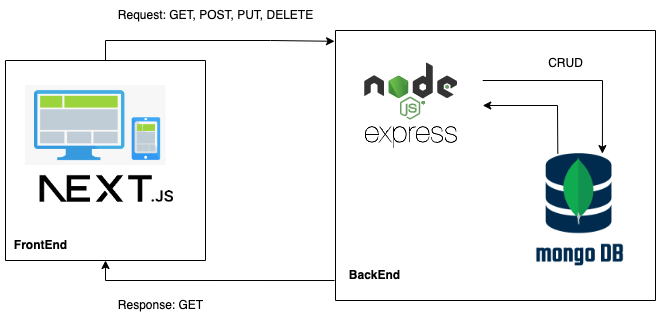
\includegraphics[width=0.8\textwidth]{latex/img/neoantigen/arquitectura.png}
	\caption{Arquitectura de la aplicación Web.}
	\label{fig:arquitectura}
\end{figure}


	
	\bibliographystyle{apalike}
	\bibliography{bibliography}

\clearpage

\section{Integrantes del equipo}
En la Tabla \ref{tab:integrantes}, presentamos al equipo de investigación.

\begin{table}[H]
\caption{Integrantes del equipo de investigación}
\label{tab:integrantes}
\begin{tabular}{p{3cm}p{2cm}p{2cm}p{2cm}p{3cm}}
\textbf{Nombre y apellidos} & \textbf{Cargo}         & \textbf{Escuela profesional} & \textbf{Rol del proyecto} & \textbf{Descripción breve del rol} \\ \hline
Vicente Machaca Arceda      & Investigador principal & Ingeniería de Software       & Investigador principal    & Investigación y desarrollo         \\
Richart Escobedo Quispe     & Co-investigador        & Ingeniería de Software       & Co-investigador           & Investigación y desarrollo         \\
Estudiante 01               & Asistente              & Ingeniería de Software       & Asistente                 & Desarrollo                         \\
Estudiante 02               & Asistente              & Ingeniería de Software       & Asistente                 & Desarrollo          \\ \hline              
\end{tabular}
\end{table}


\section{Presupuesto y cronograma}

En la Tabla \ref{tab:presupuesto}, presentamos el presupuesto para el trabajo de investigación. Este asciende a la suma de 4000 mil soles.

\begin{table}[H]
	\centering
	\setlength{\tabcolsep}{0.5em} % for the horizontal padding
	{\renewcommand{\arraystretch}{1.2}% for the vertical padding
		\caption{Presupuesto. Abreviaciones, PC: \textit{Personal Computer}}
		\label{tab:presupuesto}
		\begin{tabular}{|p{8cm}|c|c|c|} \hline
			\textbf{Insumo o material}    & \textbf{Unidades} & \textbf{Precio} & \textbf{Total} \\ \hline
			Incentivo para el investigador principal          & 1                 & 700            & 700           \\
			Incentivo para el co-investigador & 1                 & 700            & 700           \\
			Hosting y dominio                      & 1                 & 600            & 600           \\
			Workshops y cursos       & 1                 & 1000            & 1000           \\
			Servicios de \textit{cloud computing} para entrenar los modelos       & 1                 & 1000            & 1000           \\
			 \hline
			\textbf{Total}                         &                   &                 & \textbf{4000}         \\ \hline
		\end{tabular}
	}
\end{table}


En la Tabla \ref{tab:actv}, presentamos el cronograma de actividades por mes.

\begin{table}[H]
	\centering
	\setlength{\tabcolsep}{0.5em} % for the horizontal padding
	{\renewcommand{\arraystretch}{1.2}% for the vertical padding
		\caption{Cronograma de actividades por mes.}
		\label{tab:actv}
	\begin{tabular}{|p{7.8cm}|c|c|c|c|c|c|c|} \hline
		\textbf{Actividades}                                              & I & II & III & IV & V & VI & VII  \\ \hline
		
		\textbf{HITO I} & & & & & & & \\
		Revisión de la literatura                              & x                     & x                      & x                       & x                      &                       &                        &                                                  \\
		Implementación del modelo de inteligencia artificial                             &       x                &           x             &                x         & x                      &                       &                        &                                                \\
		Evaluación y comparación del modelo     &                       &                        & x                       & x                      & x                     &                        &                                                   \\
		
		\textbf{HITO II} & & & & & & & \\
		Implementación de la página Web &                       &                        &                         & x                      & x                     & x                      &                                                  \\
		Redacción del artículo de investigación                                        &                       &                        &                         &                        & x                     & x                      & x                                              \\
		Difusión de resultados                                  &                       &                        &                         &                       &                      &                       & x                                             \\ \hline
	\end{tabular}
}
\end{table}

\section{Propuesta de la conferencia o revista}

El artículo de investigación será presentado a la conferencia: ``18th International Conference on Practical Applications of Computational Biology \& Bioinformatics'' (\href{https://www.pacbb.net/}{enlace}). Está conferencia indexa los artículos en Scopus a tambien en la revista Lecture Notes in Networks and Systems que es H-index 27 según Scimago (\href{https://www.scimagojr.com/journalsearch.php?q=21100901469&tip=sid&clean=0}{enlace}). A su vez, está conferencia invita a los mejores artículos a una publicación extendida en revistas \textit{Quartil Q1}.


\section{Enlaces web de los CV de los miembros del grupo }

En la Table \ref{tab:inve}, presentamos los enlaces a los CV's del CTI vitae y el código RENACYT.

\begin{table}[H]
\centering
\caption{CV de los investigadores.}
\label{tab:inve}
\begin{tabular}{lll}
\textbf{Nombre y apellidos} & \textbf{Link CTI vitae}                                                                      & \textbf{Código RENACYT} \\ \hline
Vicente Machaca Arceda      & \href{https://dina.concytec.gob.pe/appDirectorioCTI/VerDatosInvestigador.do?id\_investigador=22551}{enlace} & P0022551                \\
Richart Escobedo Quispe     & \href{https://dina.concytec.gob.pe/appDirectorioCTI/VerDatosInvestigador.do?id\_investigador=20597}{enlace} & -     \\ \hline                 
\end{tabular}
\end{table}


	
\end{document}